\chapter{Технико-экономический раздел}
\section{Организация и планирование процесса разработки}

Организационно-экономическая часть процесса разработки программного продукта предусматривает выполнение следующих работ:
\begin{itemize}
\item формирование состава выполняемых работ и группировка их по стадиям разработки;
\item расчет трудоемкости проекта;
\item определение продолжительности выполнения отдельных этапов разработки;
\item календарный график выполнения проекта;
\item контроль выполнения календарного графика.
\end{itemize}

\subsection{Формирование состава выполняемых работ и группировка их по стадиям разработки}
Разработку программного продукта можно разделить на следующие стадии:
\small{
\begin{longtable}{|p{0.16\textwidth}|p{0.47\textwidth}|p{0.3\textwidth}|}
  \caption{Состав выполняемых работ и стадии разработки программного продукта}
  \label{tab:containsAndStages}
  \\ \hline
  \multicolumn{1}{|p{0.16\textwidth}|}{\centering Стадии разработки программного продукта}
  & \multicolumn{1}{p{0.47\textwidth}|}{\centering Состав работ, выполняемых разработчиками постановки задачи}
  & \multicolumn{1}{p{0.3\textwidth}|}{\centering Состав работ, выполняемых разработчиками программного продукта} \\
  \hline
  \endfirsthead
  \multicolumn{2}{l}{Продолжение табл.~\thetable{}} \\[0.5ex]
  \hline
  \endhead

  \hline
  \endlastfoot

    Техническое задание (ТЗ) & Постановка задач, выбор критериев эффективности. Разработка технико-экономического обоснования разработки. Выбор средств программирования. Предварительный выбор методов выполнения работы. Разработка календарного плана. & Определение состава пакета прикладных программ, состава и структуры. \\

  \hline
    Эскизный проект (ЭП) & Предварительная разработка структуры входных и выходных данных. Разработка общего описания алгоритмов реализации решения задач. Разработка пояснительной записки. Согласование и утверждение эскизного проекта. & Консультация разработчиков постановки задач. Согласование и утверждение эскизного проекта. \\

  \hline
    Технический проект (ТП) & Разработка алгоритмов решения задач. Разработка пояснительной записки. Согласование и утверждение технического проекта. Уточнение структуры, анализ и определение формы предоставления входных и выходных данных. Выбор конфигурации технических средств. & Разработка структуры программы. Разработка программной документации и передача ее для включения в технический проект. Уточнение структуры, анализ и определение формы предоставления входных и выходных данных. Выбор конфигурации технических средств. \\

  \hline
    Рабочий проект (РП) & Комплексная отладка задач и сдача в опытную эксплуатацию. Разработка проектной документации. Разработка, согласование программы и методики испытаний. Предварительное проведение испытаний. & Программирование и отладка программ. Описание контрольного примера. Разработка программной документации. Разработка, согласование программы и методики испытаний. Предварительное проведение всех испытаний. \\

  \hline
    Внедрение (В) & Подготовка и передача программной документации для сопровождения с оформлением соответствующего Акта. Передача программной продукции в фонд алгоритмов и программ. Проверка алгоритмов и программ решения задач, корректировка документации после опытной эксплуатации программного продукта. & Проверка алгоритмов и программ решения задач, корректировка документации после опытной эксплуатации программного продукта. \\
  \hline
\end{longtable}
}
\normalsize

Планирование длительности этапов и содержания проекта осуществляется в соответствии с ЕСПД~ГОСТ~34.603-92 и распределяет работы по этапам, как показано в табл.~\ref{tab:planTime}.

\begin{table}[ht]\footnotesize
  \caption{Распределение работ проекта по этапам}
  \begin{tabular}{|c|l|c|p{0.5\textwidth}|}
  \hline
  Этап &
  \multicolumn{1}{p{0.3\textwidth}|}{\centering Основные стадии} &
  \No &
  \multicolumn{1}{p{0.5\textwidth}|}{\centering Содержание работы} \\
  \hline
  \multirow{3}{*}{\centering 1} & \multirow{3}{*}{\centering Техническое задание} & 1 & Постановка задачи \\
  \cline{3-4}
   & & 2 & Анализ предметной области \\
  \cline{3-4}
   & & 3 & Выбор средств разработки, сторонних библиотек \\
  \hline


  \multirow{3}{*}{\centering 2} & \multirow{3}{*}{\centering Эскизный проект} & 4 & Разработка библиотеки голосовой аутентификации \\
  \cline{3-4}
   & & 5 & Разработка схемы хранения данных \\
  \cline{3-4}
   & & 6 & Разработка пользовательского интерфейса \\
  \cline{3-4}
   & & 7 & Разработка контроллера \\
  \hline
  \multirow{7}{*}{\centering 3} & \multirow{7}{*}{\centering Техно-рабочий проект} & 8 & Реализация алгоритмов голосовой аутентификации \\
  \cline{3-4}
   & & 9 & Реализация пользовательского интерфейса \\
  \cline{3-4}
   & & 10 & Реализация контроллера \\
  \cline{3-4}
   & & 11 & Отладка программного комплекса \\
  \cline{3-4}
   & & 12 & Экспериментальное определение параметров и характеристиксистемы \\
  \cline{3-4}
   & & 13 & Разработка документации к системе \\
  \cline{3-4}
   & & 14 & Итоговое тестирование системы \\
  \hline
  4 & \centering Внедрение & 15 & Установка и настройка программного продукта \\
  \hline
  \end{tabular}
  \label{tab:planTime}
\end{table}

\normalsize

\subsection{Расчет трудоемкости выполнения работ}
Трудоемкость разработки программной продукции зависит от ряда факторов, основными из которых являются следующие:
\begin{itemize}
\item степень новизны разрабатываемого программного комплекса;
\item сложность алгоритма его функционирования;
\item объем используемой информации, вид ее представления и способ обработки;
\item уровень используемого алгоритмического языка программирования (Чем выше уровень языка, тем меньше трудоемкость). 
\end{itemize}

Разрабатываемый программный продукт можно отнести:
\begin{itemize}
\item По степени новизны~--- к группе В. Разработка программной продукции, не имеющей аналогов.
\item По степени сложности алгоритма функционирования~--– к 3-ей группе. Разработка программной продукции, реализующей алгоритмы стандартных методов решения задач.
\item По виду представления исходная информация относится к группе 12 (исходная информация представлена в форме документов, имеющих одинаковый формат и структуру, требуется форматный контроль информации).
%to do исправить стркутуру выходных документов
\item Структура выходных документов относится к группе 22 (требуется вывод на печать одинаковых документов, вывод информационных массивов на машинные носители).
\item Количество разновидностей форм входной информации - 3.
\item Количество разновидностей форм выходной информации - 3.
\end{itemize}

Трудоемкость разработки программной продукции $\tau_{\text{ПП}}$ может быть определена как сумма величин трудоемкости выполнения отдельных стадий разработки ПП из выражения \ref{F:tauPP}.

\begin{equation}
\tau_{\text{ПП}} = \tau_{\text{ТЗ}} + \tau_{\text{ЭП}} + \tau_{\text{РП}} + \tau_{\text{В}}
\label{F:tauPP}
\end{equation}

где $\tau_{\text{ТЗ}}$~--- трудоемкость разработки технического задания на создание ПП; \\ $\tau_{\text{ЭП}}$~--- трудоемкость разработки эскизного проекта ПП; \\ $\tau_{\text{ТП}}$~--– трудоемкость разработки технического проекта ПП; \\ $\tau_{\text{РП}}$~--– трудоемкость разработки рабочего проекта ПП; \\ $\tau_{\text{В}}$~--- трудоемкость внедрения разработанного ПП.

Трудоемкость разработки технического задания рассчитывается по формуле \ref{F:tauTZ}:

\begin{equation}
\tau_{\text{ТЗ}} = {T_{\text{РЗ}}}^\text{З} + {T_{\text{РП}}}^\text{З}
\label{F:tauTZ}
\end{equation}

где ${T_{\text{РЗ}}}^\text{З}$ - затраты времени разработчика постановки задач на разработку ТЗ, чел.-дни; \\ ${T_{\text{РП}}}^\text{З}$ - затраты времени разработчика программного обеспечения на разработку ТЗ, чел.-дни.

Значения величин ${T_{\text{РЗ}}}^\text{З}$ и ${T_{\text{РП}}}^\text{З}$ рассчитываются по формулам~\ref{F:TrzZ},~\ref{F:TrpZ}:

\begin{equation}
{T_{\text{РЗ}}}^\text{З} = t_\text{З} \cdot {K_{\text{РЗ}}}^\text{З}
\label{F:TrzZ}
\end{equation}

\begin{equation}
{T_{\text{РП}}}^\text{З} = t_\text{З} \cdot {K_{\text{РП}}}^\text{З}
\label{F:TrpZ}
\end{equation}

где $t_\text{З}$~--- норма времени на разработку ТЗ на программный продукт в зависимости от функционального назначения и степени новизны разрабатываемого ПП, чел.-дни; \\ ${K_{\text{РЗ}}}^\text{З}$~--- коэффициент, учитывающий удельный вес трудоемкости работ, выполняемых разработчиком постановки на стадии ТЗ; \\ ${K_{\text{РП}}}^\text{З}$~--- коэффициент, учитывающий удельный вес трудоемкости работ, выполняемых разработчиком постановки на стадии РП.

$t_{\text{З}} = 36$ чел.-дн. (задачи расчетного характера)

${K_{\text{РЗ}}}^\text{З} = 0.65$ (совместная разработка)

${K_{\text{РП}}}^\text{З} = 0.35$ (совместная разработка)

$\tau_{\text{ТЗ}} = 36 \cdot (0.65 + 0.35) = 36 $ чел.-дн.

Аналогично, по формуле \ref{F:tauEP}, рассчитывается трудоемкость эскизного проекта ПП $\tau_{\text{ЭП}}$.

\begin{equation}
\tau_{\text{ЭП}} = {T_{\text{РЗ}}}^\text{З} + {T_{\text{РП}}}^\text{З}
\label{F:tauEP}
\end{equation}

$t_{\text{З}} = 101$ чел.-дн. (задачи расчетного характера)

${K_{\text{РЗ}}}^\text{З} = 0.65$ (совместная разработка)

${K_{\text{РП}}}^\text{З} = 0.35$ (совместная разработка)

$\tau_{\text{ТЗ}} = 101 \cdot (0.65 + 0.35) = 101 $ чел.-дн.

Трудоемкость разработки технического проекта $\tau_{\text{ТП}}$ зависит от функционального назначения программного продукта, количества разновидностей форм входной и выходной информации и определяется как сумма времени, затраченного разработчиком постановки задач  и разработчиком программного обеспечения. Эти зависимости отражает формула~\ref{F:tauTP}.

\begin{equation}
\tau_{\text{ТП}} = ({t_{\text{РЗ}}}^T + {t_{\text{РП}}}^T) \cdot K_{\text{В}} \cdot K_{\text{Р}}
\label{F:tauTP}
\end{equation}

где ${t_{\text{РЗ}}}^T$, ${t_{\text{РП}}}^T$~--- норма времени, затрачиваемого на разработку ТП разработчиком постановки задач и разработчиком программного обеспечения соответственно, чел.-дни; \\ $K_{\text{В}}$~--- коэффициент учета вида используемой информации; \\
$K_{\text{Р}}$~--- коэффициент учета режима обработки информации.

Значение коэффициента $K_{\text{В}}$ определяется из выражения:
\begin{equation}
K_{\text{В}} = \frac{K_{\text{П}} \cdot n_{\text{П}} + K_{\text{НС}} \cdot n_{\text{НС}} + K_{\text{Б}} \cdot n_{\text{Б}}}{n_{\text{П}} + n_{\text{НС}} + n_{\text{Б}}}
\label{F:Kv}
\end{equation}

где $K_{\text{П}}$, $K_{\text{НС}}$, $K_{\text{Б}}$~--– значения коэффициентов учета вида используемой информации для переменной, нормативно-справочной информации и баз данных соответственно; \\ $n_{\text{П}}$, $n_{\text{НС}}$, $n_{\text{Б}}$~--– количество наборов данных переменной, нормативно-справочной информации и баз данных соответственно.

$K_{\text{П}} = 1.2$, $K_{\text{НС}} = 1.08$, $K_{\text{Б}} = 3.12$

$n_{\text{П}} = 6$, $n_{\text{НС}} = 4$, $K_{\text{Б}} = 0$

По формуле~\ref{F:Kv}:

$K_{\text{В}} = 1.15$

$K_{\text{Р}} = 1.45$

По формуле~\ref{F:tauTP}:

$\tau_{\text{ТП}} = (14 + 12) \cdot 1.15 \cdot 1.45 = 43$ чел.-дн.

Трудоемкость разработки рабочего проекта $\tau_{\text{РП}}$ зависит от функционального назначения ПП, количества разновидностей форм входной и выходной информации, сложности алгоритма функционирования, сложности контроля информации, степени использования готовых программных модулей, уровня алгоритмического языка программирования и определяется по формуле:

\begin{equation}
\tau_{\text{РП}} = K_{\text{К}} \cdot K_{\text{Р}} \cdot K_{\text{Я}} \cdot K_{\text{З}} \cdot K_{\text{ИА}} \cdot ({t_{\text{РЗ}}}^T + {t_{\text{РП}}}^T)
\label{F:tauRP}
\end{equation}

где $K_{\text{К}}$~--– коэффициент учета сложности контроля информации; \\ $K_{\text{Я}}$~--– коэффициент учета уровня используемого алгоритмического языка программирования; \\ $K_{\text{З}}$~--– коэффициент учета степени использования готовых программных модулей; \\ $K_{\text{ИА}}$~--– коэффициент учета вида используемой информации и сложности алгоритма ПП; \\ ${t_{\text{РЗ}}}^T$, ${t_{\text{РП}}}^T$ – норма времени, затраченного на разработку РП на алгоритмическом языке высокого уровня разработчиком постановки задач и разработчиком программного обеспечения соответственно, чел.-дни.

Значение коэффициента $K_{\text{ИА}}$ определяется из выражения:
\begin{equation}
K_{\text{ИА}} = \frac{{K_{\text{П}}}' \cdot n_{\text{П}} + {K_{\text{НС}}}' \cdot n_{\text{НС}} + {K_{\text{Б}}}' \cdot n_{\text{Б}}}{n_{\text{П}} + n_{\text{НС}} + n_{\text{Б}}}
\label{F:KIA}
\end{equation}

где ${K_{\text{П}}}'$, ${K_{\text{НС}}}'$, ${K_{\text{Б}}}'$ - значения коэффициентов учета сложности алгоритма ПП и вида используемой информации для переменной, нормативно-справочной информации и баз данных соответственно.

$K_{\text{К}} = 1$

$K_{\text{Р}} = 1.52$

$K_{\text{Я}} = 1$ (алгоритмический язык высокого уровня)

$K_{\text{З}} = 0.5$ (использование более 60\% готовых программных модулей)

$\tau_{\text{РЗ}} = 14, \tau_{\text{РП}} = 12$

По формуле~\ref{F:KIA}:

$K_{\text{ИА}} = 1.01$

По формуле~\ref{F:tauRP}:

$\tau_{\text{РП}} = 44 \cdot 1 \cdot 1.52 \cdot 1 \cdot 0.5 \cdot 1.01 = 34$ чел.-дн.

Так как при разработке ПП стадии «Технический проект» и «Рабочий проект» объединены в стадию «Техно-рабочий проект», то трудоемкость ее выполнения $\tau_{\text{РП}}$ определяется по формуле:
\begin{equation}
\tau_{\text{ТРП}} = 0.85 \cdot \tau_{\text{ТП}} + \tau_{\text{РП}}
\label{F:tauTRP}
\end{equation}

Таким образом $\tau_{\text{ТРП}} = 0.85 \cdot 43 + 34 = 71$ чел.-дн.

Трудоемкость выполнения стадии внедрения $\tau_{\text{В}}$ может быть рассчитана по формуле:
\begin{equation}
\tau_{\text{В}} = ({t_{\text{РЗ}}}^\text{В} + {t_{\text{РП}}}^\text{В}) \cdot K_{\text{К}} \cdot K_{\text{Р}} \cdot K_{\text{З}}
\label{F:tauTV}
\end{equation}

где ${t_{\text{РЗ}}}^\text{В}$, ${t_{\text{РП}}}^\text{В}$ ~--- норма времени, затрачиваемого разработчиком постановки задач и разработчиком программного обеспечения соответственно на выполнение процедур внедрения ПП, чел.-дни.

${t_{\text{РЗ}}}^\text{В} = 13$, ${t_{\text{РП}}}^\text{В} = 20$

По формуле~\ref{F:tauTV}:

$\tau_{\text{В}} = (13+20) \cdot 1 \cdot 1.52 \cdot 0.5 = 25$ чел.-дн.

Подставив полученные данные в формулу~\ref{F:tauPP}, получим:

$\tau_{\text{ПП}} = 36 + 101 + 71 + 25 = 233$ чел.-дн.

\begin{table}[ht]\footnotesize
  \caption{Распределение работ проекта по этапам}
  \begin{tabular}{|c|c|p{0.23\textwidth}|c|p{0.45\textwidth}|c|}
  \hline
  \begin{sideways}Этап\end{sideways} &
  \begin{sideways}\parbox{30mm}{Трудоемкость этапа, чел.-дн.}\end{sideways} &
  \centering Основные стадии &
  \No &
  \multicolumn{1}{p{0.4\textwidth}|}{\centering Содержание работы} &
  \begin{sideways}\parbox{30mm}{Трудоемкость, чел.-дн.}\end{sideways} \\
  \hline
  \multirow{3}{*}{\centering 1} & \multirow{3}{*}{\centering 36} & \multirow{3}{0.23\textwidth}{\centering Техническое задание} & 1 & Постановка задачи & 10\\
  \cline{4-6}
   & & & 2 & Анализ предметной области & 15\\
  \cline{4-6}
   & & & 3 & Выбор средств разработки, сторонних библиотек & 11\\
  \hline
  \multirow{3}{*}{\centering 2} & \multirow{3}{*}{\centering 101} & \multirow{3}{0.23\textwidth}{\centering Эскизный проект} & 4 & Разработка библиотеки голосовой аутентификации & 40\\
  \cline{4-6}
   & & & 5 & Разработка схемы хранения данных & 13 \\
  \cline{4-6}
   & & & 6 & Разработка пользовательского интерфейса & 20 \\
  \cline{4-6}
   & & & 7 & Разработка контроллера & 28\\
  \hline
  \multirow{8}{*}{\centering 3} & \multirow{7}{*}{\centering 71} & \multirow{7}{0.23\textwidth}{\centering Техно-рабочий проект} & 8 & Реализация алгоритмов голосовой аутентификации & 10\\
  \cline{4-6}
   & & & 9 & Реализация пользовательского интерфейса & 8\\
  \cline{4-6}
   & & & 10 & Реализация контроллера & 11\\
  \cline{4-6}
   & & & 11 & Отладка программного комплекса & 11\\
  \cline{4-6}
   & & & 12 & Экспериментальное определение параметров и характеристиксистемы & 12\\
  \cline{4-6}
   & & & 13 & Разработка документации к системе & 10\\
  \cline{4-6}
   & & & 14 & Итоговое тестирование системы & 9\\
  \hline
  4 & 25 & \centering Внедрение & 15 & Установка и настройка программного продукта & 25\\
  \hline
  Всего & 233 & & & & \\
  \hline
  \end{tabular}
  \label{tab:Tstages}
\end{table}

\normalsize

\subsection{Расчет количества исполнителей}
Средняя численность исполнителей при реализации проекта разработки и внедрения ПО определяется соотношением:

\begin{equation}
N = \frac{Q_{\text{р}}}{F}
\label{F:Nispoln}
\end{equation}

где $Q_\text{р}$~--- затраты труда на выполнение проекта (разработка и внедрение ПО); \\ $F$~--- фонд рабочего времени.

Величина фонда рабочего времени определяется соотношением:

\begin{equation}
F = T \cdot F_{\text{М}}
\label{F:Ffond}
\end{equation}

где $T$~--- время выполнения проекта в месяцах, равное 5 месяцам; \\ $F_\text{М}$~--- фонд времени в текущем месяце, который рассчитывается из учета общества числа дней в году, числа выходных и праздничных дней:

\begin{equation}
F_{\text{М}} = \frac{t_{\text{р}} \cdot (D_{\text{К}} - D_{\text{В}} - D_{\text{П}})}{12}
\label{F:FMfond}
\end{equation}

где $t_{\text{р}}$~--- продолжительность рабочего дня; \\ $D_{\text{К}}$~--- общее число дней в году; \\ $D_{\text{В}}$~--- число выходных дней в году; \\ $D_{\text{П}}$~--- число праздничных дней в году.

По формуле~\ref{F:FMfond}:

$F_{\text{М}} = \frac{8 \cdot (365 - 103 - 11)}{12} = 162$

По формуле~\ref{F:Ffond}:

$F = 5 \cdot 162 = 810$

По формуле~\ref{F:Nispoln} получим число исполнителей проекта:

$N = \frac{233 \cdot 8}{810} = 3$

\subsection{Календарный план-график разработки}
Планирование и контроль хода выполнения разработки проводится по календарному графику выполнения работ.

\begin{table}[ht!]\footnotesize
  \caption{Планирование разработки}
  \begin{tabular}{|p{0.2\textwidth}|l|p{0.25\textwidth}|p{0.17\textwidth}|l|}
  \hline
  Стадия разработки & Трудоемкость & Должность исполнителя & Распределение трудоемкости & Численность \\
  \hline
  \multirow{3}{0.2\textwidth}{Техническое задание} & \multirow{3}{*}{36} & Ведущий программист & 20 (56\%) & 1\\
  & & Программист 1 & 8 & 1\\
  & & Программист 2 & 8 & 1\\
  \hline
  \multirow{3}{0.2\textwidth}{Эскизный проект} & \multirow{3}{*}{101} & Ведущий программист & 51 (51\%) & 1\\
  & & Программист 1 & 25 & 1\\
  & & Программист 2 & 25 & 1\\
  \hline
  \multirow{3}{0.2\textwidth}{Технический проект} & \multirow{3}{*}{71} & Ведущий программист & 23 (53\%) & 1\\
  & & Программист 1 & 10 & 1\\
  & & Программист 2 & 10 & 1\\
  \hline
  \multirow{3}{0.2\textwidth}{Внедрение} & \multirow{3}{*}{25} & Ведущий программист & 13 (52\%) & 1\\
  & & Программист 1 & 6 & 1\\
  & & Программист 2 & 6 & 1\\
  \hline
  Итого & 233 & & & \\
  \hline
  \end{tabular}
  \label{tab:planColletive}
\end{table}

\normalsize

\begin{table}[ht!]\footnotesize
  \caption{Календарный ленточный график работ}
  \begin{tabular}{|l|l|l l l l|}
  \hline
  Стадия разработки & Должность исполнителя & \multicolumn{4}{c|}{Трудоемкость} \\
  \hline
  \multirow{3}{0.2\textwidth}{Техническое задание} 
  & Ведущий программист & \framebox[2\width]{\mbox{ 20 }}& & & \\
  & Программист 1       & \framebox[1\width]{8} & & & \\
  & Программист 2       & \framebox[1\width]{\mbox{8}} & & & \\
  \hline
  \multirow{3}{0.2\textwidth}{Эскизный проект} 
  & Ведущий программист & & \framebox[3\width]{  51  } & & \\
  & Программист 1 & &       \framebox[1.5\width]{\mbox{25}} & & \\
  & Программист 2 & &       \framebox[1.5\width]{\mbox{25}} & & \\
  \hline
  \multirow{3}{0.2\textwidth}{Технический проект} & Ведущий программист & & & \framebox[2\width]{\mbox{  23  }} &\\
  & Программист 1 & & & \framebox[1\width]{10} & \\
  & Программист 2 & & & \framebox[1\width]{10} & \\
  \hline
  \multirow{3}{0.2\textwidth}{Внедрение} & Ведущий программист & & & & \framebox[2\width]{13} \\
  & Программист 1 & & & & \framebox[1.1\width]{6}\\
  & Программист 2 & & & & \framebox[1.1\width]{6}\\
  \hline
  \end{tabular}
  \label{tab:planColletiveTimeline}
\end{table}

\normalsize

Исходя из табл. \ref{tab:planColletiveTimeline}, при использовании оптимизации в результате параллельной работы ведущего инженера и программистов можно добиться сокращения срока разработки и внедрения программного продукта с 233 дней до 107 дней, т. е. в 2,17 раза.

\section{Определение цены программной продукции}
Затраты на выполнение проекта состоят из затрат на заработную плату исполнителям, затрат на закупку или аренду оборудования, затрат на организацию рабочих мест, и затрат на накладные расходы.
Ниже приведены затраты на заработную плату и отчисления на социальное страхование в пенсионный фонд, фонд занятости и фонд обязательного медицинского страхования (26\%). Для всех исполнителей предполагается оклад в размере 10000 рублей в месяц.

\begin{table}[ht!]\footnotesize
  \caption{Затраты на зарплату и отчисления на социальное страхование}
  \begin{tabular}{|c|l|l|l|l|l|}
  \hline
  Месяц & & \multicolumn{3}{c|}{Исполнитель} & Итого, руб.\\
  \cline{3-5}
  & & 1 & 2 & 3 &\\
  \hline
  \multirow{3}{0.2\textwidth}{Февраль} & Рабочих дней & 20 & 8 & 8 & \multirow{3}{*}{18900} \\
  & Зарплата & 8333 & 3333 & 3333 &\\
  & ЕСН & 2167 & 867 & 867 &\\
  \hline
  \multirow{3}{0.2\textwidth}{Март} & Рабочих дней & 24 & 24 & 24 & \multirow{3}{*}{37800} \\
  & Зарплата & 10000 & 10000 & 10000 &\\
  & ЕСН & 2600 & 2600 & 2600 &\\
  \hline
  \multirow{3}{0.2\textwidth}{Апрель} & Рабочих дней & 24 & 1 & 1 & \multirow{3}{*}{13650} \\
  & Зарплата & 10000 & 417 & 417 &\\
  & ЕСН & 2600 & 108 & 108 &\\
  \hline
  \multirow{3}{0.2\textwidth}{Май} & Рабочих дней & 22 & 10 & 10 & \multirow{3}{*}{22050} \\
  & Зарплата & 9167 & 4167 & 4167 &\\
  & ЕСН & 2383 & 1083 & 1083 &\\
  \hline
  \multirow{3}{0.2\textwidth}{Май} & Рабочих дней & 17 & 6 & 6 & \multirow{3}{*}{15225} \\
  & Зарплата & 7083 & 2500 & 2500 &\\
  & ЕСН & 2500 & 650 & 650 &\\
  \hline
  \multicolumn{5}{|l|}{Итого} & 107625\\
  \hline
  \end{tabular}
  \label{tab:sotsStrahZatr}
\end{table}

\normalsize

Расходы на материалы, необходимые для разработки программной продукции, указаны в табл. \ref{tab:materialsZatr}.

\begin{table}[ht!]\footnotesize
  \caption{Затраты на материалы}
  \begin{tabular}{|c|p{0.25\textwidth}|l|c|c|c|}
  \hline
  \No & Наименование & Ед. измерения & Количество & Цена за единицу, руб. & Сумма, руб.\\
  \hline
  1 & Flash USB Drive & Шт. & 1 & 400 & 400\\
  \hline
  2 & Бумага А4 & Пачка 500 л. & 1 & 100 & 100\\
  \hline
  3 & Картридж для принтера Samsung "ML-1210" & Шт. & 1 & 2300 & 2300\\
  \hline
  \multicolumn{5}{|l|}{Всего} & 2800\\
  \hline
  \end{tabular}
  \label{tab:materialsZatr}
\end{table}

\normalsize

В работе над проектом используется специальное оборудование – персональные электронно-вычислительные машины (ПЭВМ) в количестве 3 шт. Стоимость одной ПЭВМ составляет 25000 рублей. Период амортизации 36 мес.
Месячная норма амортизации рассчитывается по формуле:

\begin{equation}
K = \frac{1}{n} \cdot 100\%
\label{F:amortMonth}
\end{equation}

Таким образом:

$K = \frac{1}{36} \cdot 100\% = 2.78$ \%

За 5 месяцев работы расходы на амортизацию составят: $25000 \cdot 0.0278 \cdot 5 \cdot 3 = 10417$ руб.

Общие затраты на разработку ПП составят: $107625 + 10417 = 118042$ рублей.

\subsection{Расчет экономической эффективности}
Расчет экономической эффективности проведем, предполагая цену разработанной программной продукции 320000 рублей.
Основными показателями экономической эффективности является чистый дисконтированный доход (ЧДД) и срок окупаемости вложенных средств.
Чистый дисконтированный доход определяется по формуле:

\begin{equation}
\text{ЧДД} = \sum_{t=0}^{T} {(R_t - \text{З}_t) \cdot \frac{1}{(1 + E)^t}}
\label{F:ChDD}
\end{equation}

где $T$ – горизонт расчета по месяцам; \\ $t$ – период расчета; \\ $R_t$ – результат, достигнутый на t шаге (стоимость); \\ $\text{З}_t$ – затраты; \\ $E$ – приемлемая для инвестора норма прибыли на вложенный капитал.

Коэффициент $E$ установим равным ставке рефинансирования ЦБ РФ – 8\% годовых (или 0.67\% в месяц). В результате анализа рынка программной продукции с направленностью, аналогичной разрабатываемой, планируется продажа 2 единицы ПП каждый месяц. Планируемая цена ПП составляет 20000 рублей. Предполагаемые накладные расходы, связанные с реализацией составят 1500 рублей в месяц.

Коэффициент дисконтирования равен $K_{\text{Д}} = \frac{1}{(1 + E)} = 0.9259$.


В табл. \ref{tab:chddCalc} приведен расчет ЧДД по месяцам работы над проектом.

\pgfkeys{/pgf/number format/.cd,precision=6,use period,fixed,1000 sep={}}

\pgfplotstableread{data/chdd.dat}\chddCalc

\begin{table}[h]\footnotesize
\centering
\caption{Расчет ЧДД}
\pgfplotstabletypeset[
    columns={a,b,c,d,e}, % алиасы колонок, определённые в первой строке таблицы
    columns/a/.style={string type, column name=Месяц },
    columns/b/.style={ column name={Текущие затраты, руб.} },
    columns/c/.style={ column name={Суммарные затраты, руб.} },
    columns/d/.style={ column name={Текущий доход, руб.} },
    columns/e/.style={ column name={ЧДД, руб.} },
    every head row/.style={ before row=\hline },
    every odd row/.style={ before row=\hline },
    every even row/.style={ before row=\hline },
    every last row/.style={ after row=\hline },
    every even column/.style={
        column type/.add={|}{}
    },
    every odd column/.style={
        column type/.add={|}{}
    },
   every last column/.style={ column type/.add={}{|} }
]\chddCalc \\[0.5cm]
\label{tab:chddCalc}
\end{table}

\normalsize

\begin{figure}[ht]
\center{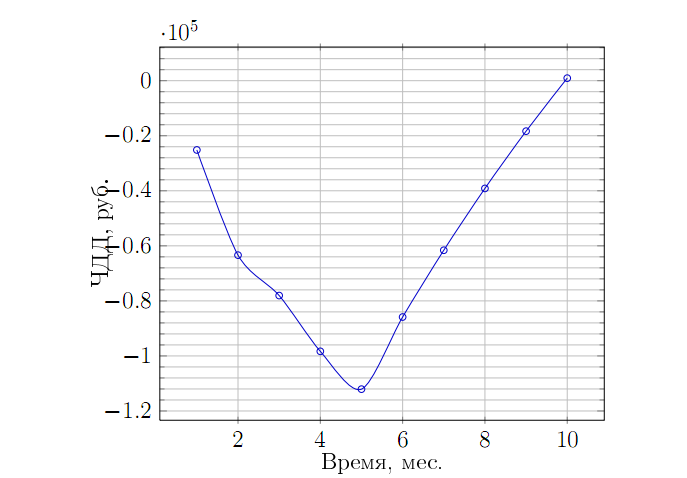
\includegraphics[scale=0.6]{static_include/economicsgr.png}}
\caption{График изменения чистого дисконтированного дохода}
\label{fig:chddGraph}
\end{figure}

\section{Вывод}
Можно прогнозировать, что проект окажется рентабельным и окупится через 5 месяцев после внедрения.
Созданный программный комплекс не имеет аналогов, реализующих все функциональные возможности комплекса. Существуют программные продукты, позволяющие производить голосовую аутентификацию, однако они нацелены на другой потребительский сектор. В силу вышесказанного, представляется довольно сложным оценить цену реализации программного средства при выдвижении на рынок. Автоматизация предметной области программного продукта началась относительно давно, рынок сбыта достаточно велик, и, предположения об окупаемости затрат на создание программы являются оптимистичными.
